%% ---------------------------------------------------------------
%% $URL: https://repository.cs.ru.is/svn/thesis-template/trunk/ruthesis/latex/DEGREE-NAME-YEAR.tex $
%% $Id: DEGREE-NAME-YEAR.tex 360 2019-02-13 22:04:35Z foley $
%% This is a template LaTeX file for dissertations, theses, or reports at Reykjavík University
%%
%% Comments and questions can be sent to the RU LaTeX group (latex AT list.ru.is)
%% ---------------------------------------------------------------

%% METHOD:
%% 0) Read ruthesis/thesis-instructions.pdf
%%    If it is missing, goto https://repository.cs.ru.is/svn/thesis-template/trunk/ruthesis/thesis-instructions.pdf
%% 0.2) Subscribe to the announcements email list at
%%    https://list.ru.is/mailman/listinfo/latex-announcements
%% 1 LaTeX instructions.tex or goto http://afs.rnd.ru.is/project/thesis-template/trunk/ruthesis/latex/instructions.pdf
%% 2) Copy the template files (or unzip) to your working area
%% 3) Rename this file (if needed) with your information e.g. MSC-FOLEY-2007.tex
%% 4) Modify this file to fit your needs (please follow all comments below in the text)
%% 5) For making bibliographies, run "biber".  You can also change
%%    this back to "bibtex".  See below in "Bibliography options".

%%%%%%% CHOOSE ONE OF THESE %%%%%%%%%%%%%%%
%% projectreport: Project report (CS)
%% bachelors: Bachelor of Science thesis
%% masters: Master of Science thesis
%% doctorate: Doctor of Philosophy dissertation
%
%%%%%%% CHOOSE ONE OF THESE %%%%%%
%%
%% draft: speed up processing by skipping graphics and adding useful
%%     information for editing.  Also sets spacing to double so that it is easier to
%%     write editing marks on paper copy.
%% proof:  proofreading version (final formatting with warnings)
%% final: generate document for submission, removing FIXMEs, and
%%     other markup.  Throw error if any fatal FIXMEs still in document.
%%
%%%%%%% CHOOSE ONE OF THESE IF APPLICABLE %%%%%%
%%
%% deptsse: School of Science and Engineering
%% deptscs: School of Computer Science
%%
%%%%%%%% CHOOSE ANY COMBINATION OF THESE %%%%%%%%%%%%
%%
%% forcegraphics: force graphics, etc. to be included, even in draft mode
%% debug:  writes more messages to the log file, adds debugging output
%%     and sizing boxes
%% icelandic: thesis is in Icelandic
%% oldstyle:  use the PhD headers and footers from the old CS template
%% online: for online versions (skip blank pages)
\documentclass[online,masters,deptscs,forcegraphics,draft]{ruthesis}

%%%%%%%%%%%%%%%%%%%% TeXStudio Magic Comments %%%%%%%%%%%%%%%%%%%%%
%% These comments that start with "!TeX" modify the way TeXStudio works
%% For details see http://texstudio.sourceforge.neit/manual/current/usermanual_en.html   Section 4.10
%%
%% What encoding is the file in?
% !TeX encoding = UTF-8
%% What language should it be spellchecked?
% !TeX spellcheck = en_US
%% What program should I compile this document with?
% !TeX program = xelatex

%%%%%%%%%%%%%%%%%%%% Bibliography options %%%%%%%%%%%%%%%%%%%%%
%% We suggest switching from bibtex to biblatex/biber because it is better able
%% to deal with Icelandic characters and other bibliography issues
%% As long as you use biblatex instead of bibtex by itself, it will at least
%%  generate a document without errors.
%% !!!If you are using TeXStudio, don't forget to update the bibliography setting!!!
\usepackage[backend=bibtex,bibencoding=utf8,style=ieee]{biblatex}
%\DeclareLanguageMapping{american}{american-apa}
% need to declare mapping for style=apa to alphabetize properly
% If you set backend=bibtex, it will use bibtex for processing (old way)
%    this can work with Icelandic characters, but you may get weird results.
%    bibtex does not know how to sort Þ and ð
% if you set backend=biber, you can use UTF8 characters such as Þ and
%     ð  but you will have to remember to switch from using bibtex to
%
%     biber in your client
% If you use JabRef, make sure the file is encoded in UTF-8 which is
%    not the default.

%% This tells TeXStudio to use biber
% !TeX TXS-program:bibliography = txs:///biber
%% This also sets the bibliography program for TeXShop and TeXWorks
% !BIB program = biber

% Where is your reference library?
\addbibresource{references.bib}

%%%%%%%%%%%%%%%%%%% CUSTOMIZATIONS %%%%%%%%%%%%%%%%%%%%%%%%%%%%%
%% It is not recommended that you customize this file nor
%% ruthesis.cls.  Just fill in the necessary fields.  You should put
%% your macros and packages into a separate file so that it is easier
%% to use updates to the template.  The custom.sty file was created
%% for this reason.  We load this much later so that it can overrite
%% any existing settings
\IfFileExists{custom.sty}{\usepackage{custom}}{}


%%%%%%%%%%%%%%% INFORMATION %%%%%%%%%%%%%%%%%%5
%% University information must be multilingual to deal with the
%%  required cover pages and abstract on thesis
%% NOTE: This may not be required for other reports!!!

%% Babel Icelandic macros are setup  on RedHat at
%% /usr/share/texlive/texmf-dist/tex/generic/babel/icelandic.sty
%% /usr/share/texlive/texmf-dist/tex/generic/babel-icelandic/icelandic.ldf


%% Multilingual macros
%\newML{macroname}{englishword}{icelandicword}
%  creates \macronameML
%    \MLmacroname[english] - returns the english word
%    \MLmacroname[icelandic] - returns the icelandic word
%    \MLmacroname  - uses the current language setting
% Some useful ones have already been defined, but can be redefined
%% Predefined: \MLIceland \MLReykjavikUniversity \MLUniversityIceland

%% What institute?  Default is RU.
%\setInstitution{\MLReykjavikUniversity}
% \newML{InstitutionAddress}{Menntavegur 1\\101 Reykjavík, Iceland}
% {Menntavegi 1\\101 Reykjavík, Ísland}
% \setInstitutionAddress{\MLInstitutionAddress}
% \newML{Tel}{Tel.}{Sími}
% \setInstitutionPhone{\MLTel{} +354 599 6200\\
% Fax +354 599 6201}
% \setInstitutionURL{www.ru.is}


%% ONLY SET DEPARTMENT IF YOU HAVE NOT USED THE deptsse or deptscs OPTION!
%% Department and degree program
%\newML{ND}{New Department}{Nytt deild}
%\setSchool{\MLND}

%% Set your program of study
\newML{program}{Computer Science}{Tölvunnarfræði}
\program{\MLprogram}

%% Degree long name.  If not already defined, you can create a macro
%\newML{DEGREE}{English Degree Name}{Icelandic Degree Name}
%% Default is set based upon doctorate vs masters option
%% Predefined: \MLMSc \MLPhd
%\setDegreelong{\MLMSc}

%% Degree abb, change if default is not right
%% Default is set based upon doctorate vs masters option
%\degreeabbrv{Sc.D.}

%\setFrontLogo{reyst-logo}
%% Use this if you need a different front logo on the first page
%% e.g. reyst-logo

%% Date in english and icelandic
%% NOTE: THIS IS THE DATE OF THE SUPERVISOR'S SIGNATURE!!!!!!
%% Predefined: \MLjan, \MLfeb, \MLmar, ... \MLdec
%\whensigned{day}{month}{year} %day is only used on some formats, but you must put something.
\whensigned{17}{\MLjan}{2021}

%% Title first in English then Icelandic
%% You need to put both a normal case and ALL CAPS version into the macros.
%%
\newML{Title}{Strategic Evaluation of Deep Neural Networks in Board Games}{Herkænsku mat á djúptauganetum í leikjum}
\newML{TITLE}{STRATEGIC EVALUATION OF DEEP NEURAL NETWORKS IN BOARD GAMES}{HERKÆNSKU MAT Á DJÚPTAUGANETUM Í LEIKJUM}
%%
\setTitle{\MLTitle}{\MLTITLE}
%% ***** Special Titles ******
%% If the title must be formatted specifically for the cover page or internal pages
%% (typically via line-breaks using the \newline command) then the following commands must be used
%%
%\setTitleCover{\MLTITLE}
%% These two for the internal cover pages, usually not needed
%\newML{TitleInternal}{Internal Title}{Icelandic Internal Title}
%\setTitleInternal{\MLTitleInternal}

%% Author name (should be the same in any language, if not use \newML)
%% If you are writing a Project report with multiple authors, separate them with \\:
%% To keep the names typeset together, you want to use non-breaking spaces: ~
%\author{Firstname1~Lastname1\\Firstname2~Lastname2}
\author{Sigurður Helgason}

%% If the name must be formatted specifically for the signature page
%% (typically via line-breaks) then the following command must be used
%\setAuthorSignature{Student\\Name}
%% This macro adjusts the author name in the headers of the oldstyle formatting
%\setAuthorHeader{StudentLast}

%%% TODO:  Move the bachelor's form separately -- it confuses people. --foley
%%%%%%%%%%%%%%%%%%%%%%%%%% Project Report or Bachelor's Only!!! %%%%%%%%%%%%%%%%%%%%%%%%%%%%%%%%%%%%%%%%%%%
\setCourse{Lokaritgerd}

%%%%%%%%%%%%%%%%%%%%%%%%%% Bachelors Only!!! %%%%%%%%%%%%%%%%%%%%%%%%%%%%%%%%%%%%%%%%%%%
\setID{270695--3459}%kennitala
\setSemester{2021--1}
\setShortSignedDate{1.1.2021}

\setOrganization{}
\setSubProgram{}

%% If the thesis is confidential, uncomment this with the date it can be released
%\setClosedDistribution{10.1.2016}%

%% Put your keywords here in English, then Icelandic.  Separate them with commas.
\newML{keywords}{Model Interpretation, Reinforcement Learning, Deep Learning, Neural Networks, Machine Learning, Game playing, Artificial Intelligence}{Djúptauganet, Tauganet, Gervigreind, Vélrænt Gagnanám}
\setKeywords{\MLkeywords}

%%%%%%%%%%%%%%%%%%%%%%%%%%% Masters Only!! %%%%%%%%%%%%%%%%%%%%%%%%%%%%%%%%%%%%%%%%%%%%
%% How many credits (ECTS) on Master's degree
%% Usually 30 or 60
\ects{60}

%%%%%%%%%%%%%%%%%%%%%%%%%%% Doctorate Only!! %%%%%%%%%%%%%%%%%%%%%%%%%%%%%%%%%%%%%%%%%%
%% Some Computer Science Thesis have an ISSN number.
%% Most other documents do not.
%\bookidnumber{ISSN: 1670-8539}
%% ID numbers are optional, but nice for sorting in libraries

%% International Standard Book Number (ISBN)
%% This is what most people should use if the thesis is being published.

%% International Standard Serial Number (ISSN)
%% This is usually only for a PhD dissertation as part of a series when published
%%   Computer Science: 1670-8539

%% Additional degrees?  (optional, usually not needed)
%\adddegree{(list of degrees in appendix)}{(sjá lista yfir prófgraður í viðauka)}
%%%%%%%%%%%%%%%%%%%%%%%%%%%%%%%%%%%%%%%%%%%%%%%%%%%%%%%%%%%%%%%%%%%%%%%%%%%%%%%%%%%%%%%%


%% List the entire committee.  Each member has a name (degree should be omitted, unless it is not PhD),
%% Supervisor(s) must appear first
%% On a Bachelors, there is usually only one supervisor and one examiner.

%% Format for each entry:
%%  \personinfo{Name}{Role}{Job Title}{Company/institution}{Country}
%% Predefined macros: \MLSupervisor \MLSupervisors \MLExaminer \MLExaminers

%% Change these to singular/plural as needed.
%% Just uncomment and change the plurality of the macro.
%\setSupervisorHeading{\MLSupervisors}
%\setExaminerHeading{\MLExaminer}

%% Predefined macros:
%% \MLSeniorProfessor \MLProfessor \MLAssociateProfessor \MLAdjunctProfessor \MLEmeritusProfessor \Iceland
%% \MLReykjavikUniversity \MLUniversityIceland

%% Bachelors: primary advisor (Umsjónarkennari), ONLY ONE!
%% All others: As many as you want
\supervisors{
  \personinfo{Yngvi Björnsson}{\MLSupervisor}{\MLProfessor}{\MLReykjavikUniversity}{\MLIceland}
%  \personinfo{Helpful A. Teacher}{Co-advisor}{\MLAssistantProfessor}{\MLUniversityIceland}{\MLIceland}
%  \personinfo{Ian M. Great}{Co-advisor}{\MLProfessor}{Hochschule Düsseldorf}{Germany}
}

%% Bachelors: secondary advisor (Leiðbeinandi), ONLY ONE
%% All others: As many as you want
\examiners{
  \personinfo{Stephan Schiffel}{\MLExaminer}{\MLAssistantProfessor}{\MLReykjavikUniversity}{\MLIceland}

  \personinfo{David Thue}{\MLExaminer}{\MLAssistantProfessor}{\MLReykjavikUniversity}{\MLIceland}
}

%% An abstract is required to be in both Icelandic and English for most degrees.
%% It is considered good form to limit the abstract to a single paragraph in each language,
%%   at 300 words.  Refer to your degree's instructions.
%% Note: Icelandic quotation marks cannot be typeset using "` and "'.  You should use \enquote{}
%% this is probably due to interactions with the MultiLingual macros.
%% TODO: turn this into more sensible macros to avoid confusion --foley
\newML{AbstractText}{\import{./sections/abstract/}{english}}{\import{./sections/abstract/}{icelandic}} % Icelandic abstract goes here
\setAbstract{\MLAbstractText}


%%%%%%%%%%%%%%INDEX SETUP %%%%%%%%%%%%%%%%%%%%%%%%%%%%%%%%%%%%%%%%%%%%%%%%%%%%
%% Indexes, and other auto-generated material
%% The Memoir package (which we use) automatically generates the index
%% See section 17.2 on page 302 of the guide
%% http://texdoc.net/texmf-dist/doc/latex/memoir/memman.pdf
%% This means you have to run "makeindex DEGREE-NAME-YEAR"
%% !!!Do not load any of the index packages, they cause problems with Memoir!!!
%% !!!You have been warned!!!
%% Note that memoir changes the [] options to only be for filenames, not other options!
\makeindex{}
\indexintoc{}

%% For abbreviations, you may want to try
%% Watch out though, each new index writes another external file and
%% latex can only write a limited number of them
%%\usepackage[intoc]{nomencl} % intoc: In Table of Contents
%% remember to run:
%% makeindex filename.nlo  -s nomencl.ist -o filename.nls

\finalifforcegraphics{hyperref} %hyperlinks even in draft mode
\usepackage[hidelinks]{hyperref}
%% !!!Must be the last package loaded except otherwise mentioned!!!!
%% \usepackage{hypcap}  %% puts link at top of figure, must be after hyperref

%%%%%%%%%%%%%%%%%%%%%%%%%%%%%%%%%%%%%%%%%%%%%%%%%%%%%%%%%%%%%%%%%%%%%%%%%%
%%%%%%%%%%%%%%%%%%%%%%% DOCUMENT START %%%%%%%%%%%%%%%%%%%%%%%%%%%%%%%%%%%
\begin{document}

%% Some elements have different names on the RU Masters rules
%% They will be annotated with RUM: "name"
\frontmatter{} % setup formatting at beginning

%\frontcover{}%%If you want to see what it looks like with the printed cover
%% TODO:  link to fill-in PDF file on RU website

\frontrequiredpages{}%% the various signaturepages and abstract
%%% WARNING:  if you get an error on the previous line, it is probably because
%%% you put a bad macro or something strange in a title, author, or abstract.

\ifdraft{\coverchapter{Important!!!  Read the Instructions!!!} If you
  have not already done so, \LaTeX{} the \path{instructions.tex} to
  learn how to setup your document and use some of the features.  You
  can see a (somewhat recent) rendered PDF of the instructions included in this folder at \path{instructions-publish.pdf}.
  There is also more information on working with \LaTeX{} at
  \url{http://samvinna.ru.is/project/htgaru/how-to-get-around-projects-publish.pdf}.
  This includes common problems and fixes.

  This page will disappear in anything other than draft mode.}{}



%% Dedication is optional, comment out if it is absent
\begin{dedications}
  I dedicate this thesis to my family who while not understanding most of what I do
  always support me. The friends that still want to talk to me even though my
  schedule has rendered me unmeetupwithable. Lastly but certainly not least,
  Hulda Lilja who always easead my mind during my spurts of imposter syndrome, and fear of
  failure.

  Don't Panic.
\end{dedications}

\enableindents{}% turn on/off paragraph indents
\coverchapter{Acknowledgements} 
\begin{quotation}
So long, and thanks for all the fish.
\end{quotation}
\vspace{\baselineskip}

\draftnote{Acknowledgements are optional; comment this chapter out if they are absent
  Note that it is important to acknowledge any funding that helped in the work}

This work was funded by \the\year~RANNIS grant ``Survey of man-eating Minke whales'' 1415550.
Additional equipment was generously donated by the Icelandic Tourism Board.

\coverchapter{Preface}

This dissertation is original work by the author, Sigurður Helgason.

  
\draftnote{The preface is an optional element
  explaining a little who performed what work.  See
  \url{https://www.grad.ubc.ca/sites/default/files/materials/thesis_sample_prefaces.pdf}
  for suggestions.
  
  List of publications as part of the preface is
  optional unless elements of the work have already been published.
  It should be a comprehensive list of all publications in which
  material in the thesis has appeared, preferably with references to
  sections as appropriate.  This is also a good place to state
  contribution of student and contribution of others to the work
  represented in the thesis.}

%\coverchapter{Publications}
%% RUM: Not mentioned, this was found in the CS thesis template.  
%% Maybe more applicable to PhD dissertations?
%%% Probably a duplication from before Preface became standard.

\starttables{}% setup formatting
%% TOC, list of figures and list of tables are required
\tableofcontents{}\clearpage%%RUM: "Table of contents"
\listoffigures{}\clearpage%%RUM: "List of figures"
\listoftables{}\clearpage%%RUM: "List of tables"

%\coverchapter{List of drawings and enclosed material}
%RUM: "List of drawings and enclosed material, e.g. CD(as appropriate)"

\listoffixmes{}
% if using fixme package, lists what needs to be done

%% The list of abbreviations is an example of a special list
%% Other lists may be added, such as lists of algorithms, symbols, theorems, etc.
%% IN CS PhD, this is sometimes centered.
\coverchapter{List of Abbreviations}%%RUM: Not mentioned
\begin{tabular}{ll}
MSc &Masters of Science\\
ML & Machine Learning\\
AI & Artificial Intelligence\\
\end{tabular}

%% This command prepares for the actual text, e.g. by
%% calling \mainmatter{}
\starttext{}

%% ---------------------------------------------------------------
%% From this point on, it is standard Latex, except the very end.
%% This is a "report"-based template, so the top-level heading
%% is \chapter{}

%% WARNING: Make sure that all of these files (and any new ones)
%% are UTF-8 otherwise you will get weird encoding errors.
%\part{The First Part} % Parts optional but useful in longer documents


%% The default division is IMRAD, you may want to divide differently
%% See the introduction for guidance.

\chapter{Introduction\label{cha:introduction}}
%% \ifdraft only shows the text in the first argument if you are in draft mode.
%% These directions will disappear in other modes.

The world of deep learning (DL) is exciting, we have models that can examine
images and very reliably be able to identify it's content. Deep learning models have
beaten Ophthalmologists in identifying diabetic retinopathy, they've identified
cancer cells where others have not. Deep learning models are used for the bleeding
edge of protein folding, to gain further understanding of the underlying structure of organisms, such as, viruses. \cite{deepmind:alphafold}
These models have done these things extremely accurately, cheap, and fast.

DL in conjunction with a randomized State-space Search Algorithm Monte-Carlo Tree Search was used to defeat the standing world champion Lee Sedol (CITE ALPHAGO ZERO) in the incredibly expansive game of Go. This was done in the year 2017, the researchers used reinforcement learning (RL), where the agent learned by only playing against itself.
These results imply that given enough time to learn the computer agent can gain a deep insight into how the game should be played.

The field of examining deep learning models to gain a richer understanding
of how they work, and what makes them so much better than humans at various tasks
is still new. This is the field of Explainable Artificial Intelligence (XAI).
If we wish to continue using artificial intelligence (AI) and machine learning (ML),
to improve our lives we must examine how they work, this is not only to improve
the models themselves but could also augment our ability in many cases.
Furthermore, these explanations are a legal requirement now in many areas\cite{legalexplanation:goodman}, namely, legal, and
medical. Recently, XAI has generally been focused on Model Interpretability (MI), in
particular, interpreting the model in such a way that we might predict what the model will
do given a particular input. Another class of XAI would be Model Explainability (ME), where we can adequately explain how the internal mechanics of the model works.
A simple example of when we're able to apply ME would be when we print out a decision tree
that is generated from an ML algorithm, with the decision tree nodes and is conditions we can see exactly what the tree will do with a given input. While in MI we would have to predict the results, without going into details as to why.

In this thesis, we take a look at how we can examine an artificial neural network (ANN)
to understand which higher-level concepts (HLC) it deems important for a given state
within games. These games can be simple like Tic-Tac-Toe or Breakthrough and extremely
complicated like Chess or Go.

The method of examining HLC's within games has generally been done by examining the
current state of the game by evaluating them concerning some heuristic. A heuristic within games are evaluations of the end reward for a state given only the state, for example,
the number of pieces left within a game of chess. Intuitively, the amount of pieces
left is a good estimate for a state in chess, this is a higher-level concept we
use to evaluate a chess position. The piece amount can be considered as a lower-level concept
than other concepts we use. For instance, grandmaster chess players evaluate a position w.r.t. states
where the king is safe from attack or the structure of the pawn positions.
This paper examines the evaluation of a neural network of a state regarding those higher-level concepts if human players evaluate the king's safety of a state
low but the neural network highly values it, and the neural network plays better
than the player. There could be an avenue for us to improve our game by considering king safety more thoroughly.

We define the research questions:

\begin{enumerate}
  \item Given a NN that plays Breakthrough very well, can we evaluate if that NN recognizes the
        HLCs that human players use.
  \item Does a NN that trains itself using self-play learn some HLCs over time, and does it start to emphasize
        the HLCs that are generally considered better, more as it trains more, and oppositely does it start to
        demphasize HLCs that are considered worse.
\end{enumerate}

\subsection{Summary of the thesis}

In this thesis, we take an example game of Breakthrough, train a neural network to play the game using only self-play. That is, the neural network is trained only by playing against itself with no outside input other than the rules of the game itself. And we examine the neural networks against popular Higher-level concepts (heuristics) that we use to play the game.
%%RUM: Introduction
\chapter{Background\label{cha:background}}

In this chapter we discuss the algorithms we decided to use, what some other similar 
methods exsist as well as the field in general.

\section{Environments}
\label{sec:environments}

When doing research on Artificial Intelligence it is important to select 
an environment that is a suitable abstraction for the task at hand. Environments vary 
significantly, and can be identified by their characteristic. The characteristics 
that are generally used to describe environments can be seen in Table \ref{tab:env_characteristics}. 
CITE AIMABOOK

\begin{table}[h]
  \centering
  \begin{tabular}{|c|c|p{6cm}|}
    \hline
    \textbf{characteristic} & \textbf{Values} & \textbf{Description}\\
    \hline
    Observable & Fully, Partially & How much of the environment can your agent percieve.\\
    \hline
    Agents & Single, Multi & Are there multiple agents playing in the environment.\\
    \hline
    Deterministic & Deterministic, Stochastic & Do the actions your agent do deterministicly impact the environment\\
    \hline
    Episodic & Sequential, Episodic & Are actions episodic or sequential\\
    \hline
    Static & Static, Semi-Static, Dynamic & ehh  \\
    \hline
    Discrete & Discrete, Continious & Is your environment discrete w.r.t actions (does it end) \\
    \hline
  \end{tabular}
  \caption{Charcteristics of environments}
  \label{tab:env_characteristics}
\end{table}

Categorizing environments like this gives you the power to find an environment in which 
a method works and know it can be applied to different environments with the same characteristics.
Talk about \textbf{agents} in the context of environments as the entities that act within the 
environment. A game player is an agent as well as the neural network model that exists within 
a car that is able to drive in the real world.

\section{Game Environment}

With classical Artificial Intelligence Game Environments are commonly used to validate a method, 
game environments can be games like Tic-Tac-Toe, Breakthrough, and driving simulators. Game environments 
are a suitable place to apply AI as they serve an important function as an abstraction of the real 
world, for instance, a self-driving car agent who is verified to avoid driving into walls in a 
simulation is possibly safer than one who is not.

\section{Breakthrough}


The game breakthrough is a simplified version of chess, the game is set up on an $MxN$ board with 
cells like in chess, and each player starts with two rows of pawns at either end. The objective of the 
game is to move one of the pawn pieces to the opposite end of the board. A player wins if 
either they have reached the opposite end of the board, or has captured all of his opponents pawns.
The pawns differ from chess pawns in such a way that they can not move two squares on the first move and,
they can move diagonally as well as forward, this leads to the game being impossible to draw as 
pieces are always able to move. An example of an initial board in breakthrough can be seen in Figure \ref{fig:initbtboard}

\begin{figure}[]
  \centering

  \breakthrough{8/8/pppppp2/pppppp2/8/8/PPPPPP2/PPPPPP2 w - - 0 1}
  
  \caption{Example breakthrough board}
  \label{fig:initbtboard}
\end{figure}


\begin{table}[h]
  \centering
  \begin{tabular}{|c|c|}\hline
    \textbf{Characteristic} & \textbf{Value}\\\hline
    Observable & Fully \\
    Agents & Multi \\
    Deterministic & Deterministic\\
    Episodic & Sequential \\
    Static & Static \\
    Discrete & Discrete \\\hline
  \end{tabular}
  \caption{Categorization of Breakthrough}
  \label{tab:breakthrough_cat}
\end{table}

Categorizing Breakthrough with the characteristics described in Section \ref{sec:environments}. We end up with the description 
shown in Table \ref{tab:breakthrough_cat}. This description is identical to that of Tic-Tac-Toe, and Chess.
This description is the most common in board games where two player compete. 

\subsection{Heuristics of Breakthrough}

To evaluate the game of Breakthrough we can consider many heuristics (higher-level concepts) for instance 
a very simple heuristic would be the amount of pieces each player has left. This heuristics gives us some 
insight into how well the game is progressing, but obviously there are cases where this doesn't tell us 
much, as in cases when your opponent has a single piece left that is on the row immediately before the 
row needed for him to win. No matter how many pieces you have left, this state is bad for you if you're not 
able to capture that piece. An example of such a state can be seen in Figure \ref{fig:bt_h1_bad}.

\begin{figure}[]
  \centering
  \breakthrough{8/8/pppp4/pp3P2/2p5/8/8/PPP5 w - - 0 1}
  \caption{Breakthrough board where Heuristic 1 doesn't work well}
  \label{fig:bt_h1_bad}
\end{figure}


A different heuristic would be the distance of your most advanced pawn minus your opponents most 
advanced pawn, this heuristic could give you insight into how close you are to winning the game or 
how close your opponent is. As a higher level concept we can call this concept your aggressiveness, 
as it closely resembles how aggressive you are for going in for the win. Generally in Breakthrough 
it is favourable to move your whole team as a unit and play more defensively, so this heuristic 
is probably not one that will lead to the most wins.

\section{State-Space Search}

Traditionally methods for playing games were searching through the environment using a heuristic to
guide the search. A simple way of doing a heuristic based search would be to give all states a $0$ 
as a score and give states where you win a positive score. We say that those search algorithm 
is not guided, and the algorithm will probably have to evaluate every state in the state-space. 
This method of searching is generally extremenly inefficient as the state-spaces of game environments 
are generally extremely large, and often infinite. For instance an estimate of the state-space 
for the game breakthrough is $M * N * 2^{N*4}$ where $M$ is the height of the board $N$ is the width 
of the board. The $2^{N*4}$ represent each piece either being alive or captured. So for a small board
$5x4$ the estimated state-space is $1310720$ many states.

This is why a good heuristic is very valuable because we can disregard all states $S'$ that 
result from doing a move $a$ in state $S$ as they will only lead to worse outcomes.

The algorithms that are used in traditional state-space search are for instance Depth-first search (DFS),
Breadth-first Search (BFS), Alpha* Search (A-Star), and Monte-Carlo Tree Search (MCTS).

More modernly these search methods have been amplified by Machine Learning, in such a way that 
we do not need to figure out a good heuristic for a given state, but rather, we apply a machine 
learning model to learn a function that takes in a state and returns an evaluation of that state.
This can lead to a significant time reduction as we do not need to simulate a whole game from a 
state to recieve its evaluation we rather receive the evaluation from the model.

\subsection{Monte-Carlo Tree Search}

\label{sec:mcts}

In the algorithm Monte-Carlo Tree Search there is an agent exists
within some environment. Where each node in the environment represents a state-action pair of the environment, by
state-action pair what is meant it is some state and the action that brought the agent to
that state. This pair should be unique within the environment. We will discuss these concepts within game-environments
and therefore we might say player instead of agent and game instead of environment.

MCTS is a method of exploring an enviroment in a randomized manner (Monte Carlo is the term implying
randomness). In MCTS there are four stages. Selection, Expansion, Simulation, and Backpropagation. They happen sequentially
and repeatedly. MCTS is initialized with a tree consisting of the unexpanded initial state of the environment.

In MCTS there is a tree representing the game-environment. This tree consists of nodes $n_i$ where $i$ represents the point in time
of the node, for example $N_0$ in chess is the initial position and $N_x$ is some position in the middle of the game and $N_e$ is one of
the states representing a position where there is either a draw or one player has won the match. Each of the nodes has $4$ values,
$s$, $a$, $Q$, and $N$. These values represent these items, $s$ is state of the environment, $a$ is the action that brought
the previous node $n_(i-1)$ to node $n_i$, $Q$ is the average value of the node (value meaning the outcome of the game),
and $N$ the amount of times the MCTS algorithm has visited this node. The values $s$ and $a$ uniquely identify a position
in the environment and are often called state-action pairs.

The MCTS algorithms four phases
\begin{enumerate}
  \item Selection
  \item Expansion
  \item Simulation/Rollout
  \item Backpropagation
\end{enumerate}


\begin{equation} \label{UCT_formula}
  \text{Child UCT value} = \frac{Q_{(s',a')}}{N_{(s',a')}} + c_{uct} * \frac{\sqrt{log(N_{(s,a)})}}{N_{(s',a')}}
\end{equation}

\subsection*{Selection}
During the selection phase a node $(s,a)$ within the tree which has not yet been expanded is found.
This process uses Upper Confidence Bound on Trees (UCT) to find that node $(s,a)$, the formula is described in Equation \ref{UCT_formula}. For a parent node $(s,a)$
(initially the root of the tree) we select the child with the highest UCT value. Repeatedly until an unexpanded
node is found. This process is done to balance the amount of exploration vs exploitation of nodes in the
tree.

\subsection*{Expansion}
Then the expansion phase expands the node generating all of $(s,a)$'s children $(s',a')$ are generated
and connected to $(s,a)$. This is done by applying all actions $a'$ to $(s,a)$. These children are the
product of applying each action $a'$ to $s$ in the parent node.

\subsection*{Rollout}
Next during rollout actions from $(s,a)$ are randomly selected to move to $(s',a')$, then repeated
to go to $(s'',a'')$, until a terminal node within the environment is reached. By terminal we mean a
state in which the game is finished. A terminal node in MCTS can generally return any value, but in the
context of this paper we only return (+1 white wins, -1 black wins, 0 draw).


\subsection*{Backpropagation}
The result from the terminal node is then propagated up through the path taken by selection $(s,a)$ up
to the root of the tree, updating the $Q_{(s,a)}$ values of each node $(s,a)$.

When training a neural network the UCT formula is modified slightly to prefer selecting nodes
that the neural network values highly by introducing a second scalar to the formula $f(s,a) = (p,v)$,
the resulting formula is described in Equation \ref{PUCT_formula}, and is called PUCT. Secondly, the backpropagation process
is modified to instead of doing rollout/simulation to recieve a reward the predicted value $v$ from
the neural network is used instead.

\begin{equation} \label{PUCT_formula}
  \text{Child PUCT value} = \frac{Q_{(s',a')}}{N_{(s',a')}} + c_{uct} * P((s,a)) * \frac{\sqrt{log(N_{(s,a)})}}{N_{(s',a')}}
\end{equation}

\section{Machine Learning}

Machine learning (ML) focuses on the using of data and a corresponding outcome w.r.t that data to 
extrapolate some underlying function of that data. This some task like predicting the 
rise and fall of some stock, what the weather will be in a week, and whether an image 
is an image of a dog or a cat. Many datastructures and algorithms are used to achieve this 
goal, but recently the field of ANN/DNN's has been the standard for achieveing the best
results.

\subsection{Reinforcement Learning}

Reinforcement Learning is a subfield of Machine Learning where a model learns from experience.
That is, the notion of input/output values changes, the model uses itself to generate input
values by acting in an environment. The environment then returns some result, that could be
losing in a game, making a correct prediction, or any number of outcomes. The result is then
propagated through the model allowing it to improve with this new information.
% When doing moving it's parameters in the direction of the recieved output
% from the environment.

Many algorithms are popular in reinforcement learning, for instance Q-learning(CITE ME), CARLA (CITE ME), 
and many others. 

\subsection{Neural Networks}

Neural networks (NN) are popular methods within a subfield of ML which is called Deep Learning (DL). 
NN's are created to resemble how the human brain functions. In the brain we have neurons which 
when they get a signal they apply some function to them and if the resulting signal is high 
enough, they fire to the next neuron. This is how it is done in the neural network model as well.
There we have neurons that when they get some input, generally a vector of numbers. The neuron 
takes the sum of that vector, weights the sum by a constant, then applies a non-linear activation 
function to it. The result of doing this is then passed on to the next neuron. Until a final layer 
of neurons is reached. At that point we have a value that the neural network corresponds to the 
input value. This value can be a binary classification (cat or dog image), a regression value (the 
value of a property), or any number of outputs. It can then be said that a neural network is doing 
a function approximation of an input to some value. $f_n ( w_n * f_{n-1} (w_{n-1} * \dots f_0(w_0*i))) = o$. 

Neural networks are machine learning models that take in as input anything that is numerical 
and they apply differentiatable function to that input s.t. they end with some output. This 
output is then compared to the expected output the difference between these outputs is called 
a loss. A loss is backpropagated through the neural network, and each function is derived in 
order to find its slope. We can then modify the weights of the neural network in the direction 
of the correct output. Leading to a function approximation of this function
$f_{neuralnetwork}(X_{input}) = O_{expectedoutput}$

\section{Explainable Artificial Intelligence (XAI)}

The field of XAI research is still very far behind it's counterpart AI research,
within XAI two fields are concidered the largest that is Model Interpretability
and Model Explainability.

\subsection{Model Interpretability}


\subsubsection{Saliency Maps}
Within XAI many methods have been developed to try to evaluate
ANN's, these methods are often referred as model interpretability methods.
In the field image recognition there has been a lot of work examining which
pixels of an image the model deems important. Arguably the most popular
method for this is Saliency Maps (CITE ME). There the pixel values the model
deems important are colored in s.t. a human can examine the image and get a
sense of what portions of the image are important to the model, an example of
a classification of a dog can be seen in Figure \ref{fig:dog_saliency}.

\begin{figure}[]
  \centering
  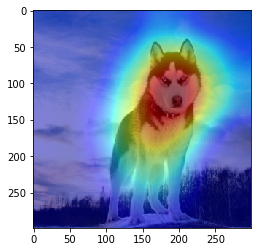
\includegraphics[width=.5\textwidth]{graphics/dog_saliency}
  \caption{Example of a models saliency map for an image of a dog}
  \label{fig:dog_saliency}
\end{figure}

While this method is understandable in the context of image recognition it
lacks severely when your input is not an image.

\subsubsection{Shapley Values}

Methods for explaining models that aren't image recognition models include
shapley values. There the input is examined against it's output, then iteratively
input values are selected to be fixed. Then the other input values are varied and
an average change in prediction is calculated. With this the shapley value can be
estimated for the fixed input value. This is done to examine which input values have
the strongest link to the output value. Shapley values on a dataset can give insights
on which input values the model deems important.

\subsubsection{Concept Activation Vectors}

A recent paper by Been Kim Et. al (CITATION NEEDED), shows a method for examining
a neural network giving a much more human insight into a prediction. Using Concept
Activation Vectors (CAV) a directional derivative for a given input can be examined
with respect to some HLC's. For example, when a human looks at an image of an animal
and is supposed to decide whether the image is of a horse or a zebra, an intuitive
approach would be to check whether the animal has stipes, or is both white and black.
That method of determining if a horse is a zebra could then be called a higher-level
concept, and if we're able to gather if a nerual network uses this strategy for prediction 
we have a deeper understanding of its underlying structure. Leading to an explanation of 
the result.

CAV's in neural networks are just binary classifiers of the same dataset used to train
a neural network. The 

\subsection{Model Explainability}

Model explainability within the context of neural networks isn't possible today. Model
explainability referrs to firstly considering some input and output from a model. Then
afterwards the model is examined to determine exactly what led to the predicted output.
This concept is simple when we're working with Decision Trees. A decision tree is a tree
whose nodes are representative of an input value and at every node a branch is selected
based on the value of the input value. It is therefore easy to see how to examine the tree
to explain the output. We just follow the branches in the tree. That being said the branches
are created by algorithms like ID3 which construct branches based on the initial dataset used
to construct the tree, but again ID3 follows simple statistics and can be explained properly.

When we talk about neural networks this process is much more difficult, the underlying nodes
are generally in the thousands, the different layers of the neural network varies in the operations
it applies to the input value and such while travelling through the neural network the modified
value becomes far removed from the initial input value to the eyes of the reader. That being said,
while the possibility of completely monitoring the training process and completely monitoring the
evaluation process is truly possible it is not feasible. And secondly the process of seeing an
input and it's corresponding output will not be of any value if one were to consider the process
of prediction.

%%RUM: Background
\chapter{Methods}

To train neural networks to play breakthrough we employ a process of self play, where two neural networks are first
randomly initialized, then they play against each other. They play for $1000$ games, and the neural network that wins
lets call that one more games is called $m_1$ and the other $M_2$. $M_1$'s weights are then copied to $M_2$. Then $M_1$,
plays against itself for $20$ iterations recording the outcome of the game. The outcome is compiled to a dataset containing
four values ($b$, $p$, $v$, $r$). $b$ stands for a gamestate within it's simulation while playing against itself, $p$ stands
for the policy returned by the neural network by 

\section{Monte Carlo Tree Search}



%\section{Machine learning methods}

This section discusses the various machine learning methods utilized throughout this project 
and discusses their applicability.

%\subsection{Deep neural network}

I'm a little teapot

%\subsection{Data joined network}

I'm a smaller teapot
%%RUM: "Methods"
\chapter{Results}

\label{cha:results}

In this chapter, we first evaluate the neural network against various agents to validate that it has learned how to play the game. Secondly, we describe each concept we intend to examine the neural network against. Thirdly, we take a look at the changes in the emphasis of the neural network during training. The main point of interest there being whether the neural network notices simple HLCs early then stops considering them as the network improves.

\section{Evolution of the Neural Networks Win Rate}

\begin{figure}
    \begin{small}
        \begin{center}
            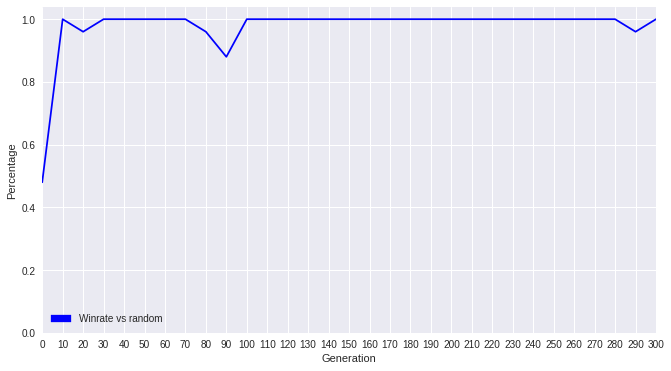
\includegraphics[width=0.7\textwidth]{graphics/winratevsrandom.png}
        \end{center}
        \caption{Winrate vs. random agent}
        \label{fig:winratevsrandom}
    \end{small}
\end{figure}

\begin{figure}
    \begin{small}
        \begin{center}
            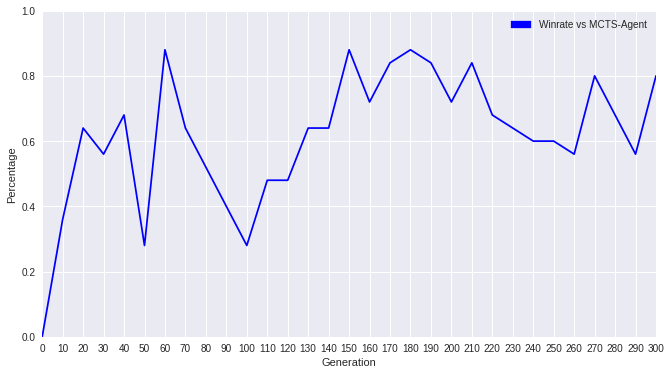
\includegraphics[width=0.7\textwidth]{graphics/winratevsmcts.png}
        \end{center}
        \caption{Winrate vs. MCTS agent}
        \label{fig:winratevsmcts}
    \end{small}
\end{figure}

\begin{figure}
    \begin{small}
        \begin{center}
            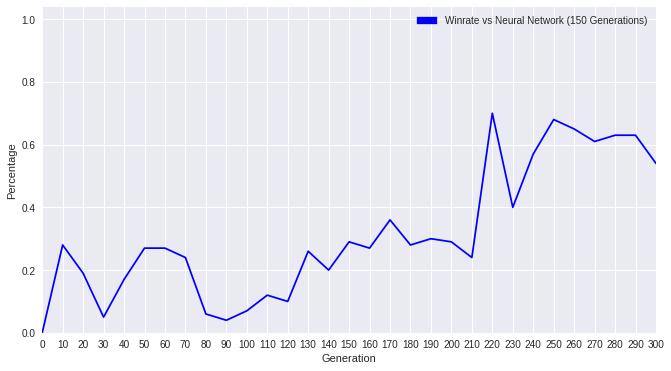
\includegraphics[width=0.7\textwidth]{graphics/winratevsneuralnetwork.png}
        \end{center}
        \caption{Winrate vs. neural network trained for 150 generations}
        \label{fig:winratevsneuralnetwork}
    \end{small}
\end{figure}

Examining the neural network is only interesting if the neural network can effectively play the game. We first examine the history of the neural network playing against an agent that only takes random moves. The win rate over every $10$ generations can be seen in Figure \ref{fig:winratevsrandom}. It is clear that very early on in the training process, almost immediately after generation $10$, our agent performs nearly perfectly against the random agent. This implies that the agent does indeed learn some strategy in the game. The next agent we tried the neural network against was an agent that does regular Monte-Carlo tree search on the game space with $100$ iterations of random UCT rollout for each move. The MCTS agent has a $c_{uct}$ value of $0.9$. A graph showing the win rate over generations is depicted in Figure \ref{fig:winratevsmcts}. Again, our agent quickly learns some strategy and can win often, although not achieving a perfect win rate even after $300$ generations. The last agent we tested against was the neural network itself, although only trained to $150$ generations. The graph in Figure \ref{fig:winratevsneuralnetwork} shows win rate. As one would expect, the agent that has trained for less time performs poorly until it has trained for more than $150$ generations.

These results imply that our agent certainly understands how to play the game of Breakthrough to a certain level. However, an intermediate level human player would most often be able to beat the agent, based on the author's experience playing against it. Note that the main focus of this was not to create an expert level agent. Rather, to gauge into the concepts the agent learns as described in the next section.

\section{Evaluating the Improvements of the Neural Network over Generations}

To test which HLC the neural network places its emphasis on during training we trained a neural network for $300$ generations, taking snapshots of the network every $10$ generations. We then had the neural network play against itself for $100$ games, collecting the states it encountered during play. These states were then examined by a concept activation vector representing these HLCs.

We test four concepts \textit{Material Advantage}, \textit{Aggressiveness}, \textit{Unity}, and \textit{Lorentz-Horey score}.

\subsection{Description of Concepts}

\begin{figure}
    \begin{small}
        \begin{center}
            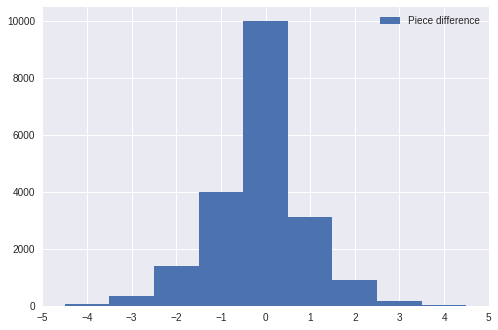
\includegraphics[width=0.95\textwidth]{graphics/dist_number_adv}
        \end{center}
    \end{small}
    \caption{Distribution of piece amount difference}
    \label{fig:distnumberadv}
\end{figure}

The first concept we examine is Material Advantage which conveys the idea of having more pawns than the opponent. When faced with a board it is difficult to argue for whether having a single pawn or three up on your opponent constitues as significant Material Advantage. In order to select an appropriate value for this case we used the neural network that had been trained for $300$ generations to generate $20{,}000$ unique states. The distribution of these states' difference of pawns can be seen in Figure \ref{fig:distnumberadv}. From examining the distribution and examining samples we selected the breakpoint of $\geq 2$, meaning that if you have $2$ pieces on your opponent you are in a state that has this concept. From the $20{,}000$ states only $5.5\%$ of states have this concept.

\begin{figure}
    \begin{small}
        \begin{center}
            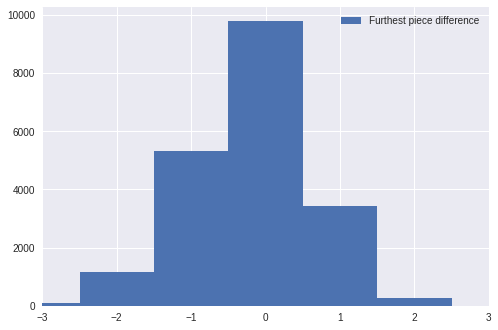
\includegraphics[width=0.95\textwidth]{graphics/dist_aggressiveness}
        \end{center}
        \caption{Distribution of difference of furthest pawns}
        \label{fig:distaggressiveness}
    \end{small}
\end{figure}

The next concept is Aggressiveness, which describes how much closer your furthest piece is to the opponent's edge than your opponent's furthest piece to your edge. This is the minimum amount of how many moves it will take you to possibly win the game. A distribution of these values can be seen in Figure \ref{fig:distaggressiveness}. We examined the distribution, and sampled states from various breaking points and decided on the value of $\geq 1$. That is, if the value of a state's furthest piece difference is greater than or equal to $1$ that state has the concept of Aggressiveness. From the dataset $18.3\%$ of states have this concept.

\begin{figure}
    \begin{small}
        \begin{center}
            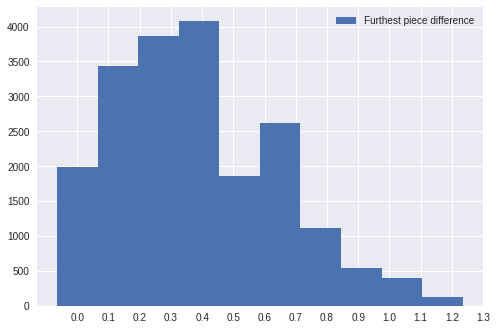
\includegraphics[width=0.95\textwidth]{graphics/dist_unity}
        \end{center}
        \caption{Difference of distance from center}
        \label{fig:distunity}
    \end{small}
\end{figure}

Our third concept is Unity. This concept represents the absolute average distance of your pawns from the center row of your pawns, and is calculated as follows: the row of your furthest pawn from the starting row $r_{far}$, the row of your nearest pawn from the starting row $r_{near}$. Finding the middle row is then $\frac{r_{far} + r_{near}}{2}$, we then take the absolute of the average distance from all of the players pawns to that row. The distribution of the average distance values is shown in Figure \ref{fig:distunity}. From sampling states from several points we decided on a breakpoint of $\le 0.25$ for identifying states as states where the Unity concept is precent. The value of $0.25$ generally allows your states to have two rows that have the majority of the pawns and one or two pawns one row away from the group. From the dataset of 20,000 states $20\%$ of states have this concept.

\begin{figure}
    \begin{small}
        \begin{center}
            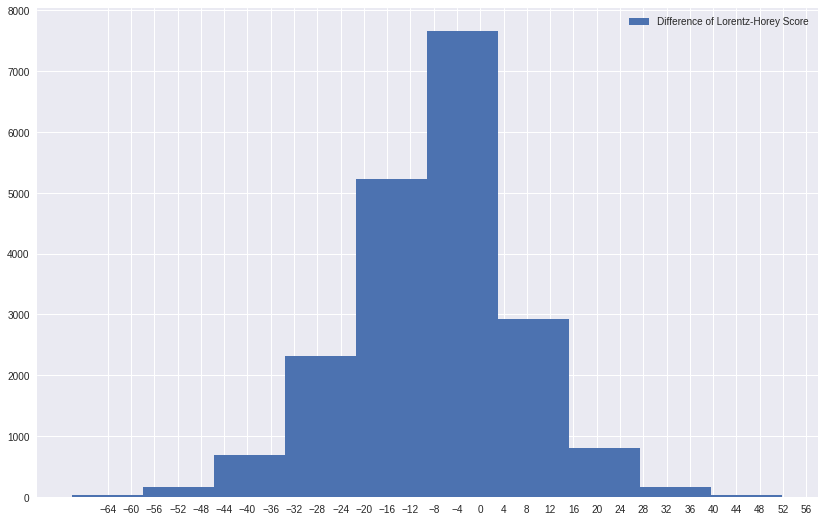
\includegraphics[width=0.95\textwidth]{graphics/dist_lorentz}
        \end{center}
        \caption{Difference of Lorentz-Horey Score}
        \label{fig:distlorentz}
    \end{small}
\end{figure}

\begin{table}[]
    \centering
    \caption{Lorentz-Horey cell values, from white players point of view}
    \begin{tabular}{|c|c|c|c|c|c|}
        \hline
        21 & 21 & 21 & 21 & 21 & 21 \\\hline
        11 & 15 & 15 & 15 & 15 & 11 \\\hline
        7  & 10 & 10 & 10 & 10 & 7  \\\hline
        4  & 6  & 6  & 6  & 6  & 4  \\\hline
        2  & 3  & 3  & 3  & 3  & 2  \\\hline
        5  & 15 & 5  & 5  & 15 & 5  \\\hline
    \end{tabular}
    \label{table:lorentzcell}
\end{table}

\label{section:lorentzhoreyref}

The last concept we examined was the Lorentz-Horey score. This concept is a popular heuristic in Breakthrough defined in the paper by Lorentz \& Horey \cite{lorentz:heuristic}. For this heuristic, we give each cell on the board a point value. For a given player the heuristic is then the sum of the cell values where they have pawns. The cell values are shown in Table \ref{table:lorentzcell}. The matrix shown is flipped from the black player's point of view. The values are selected in such a way that as your pawns approach the opponent's side their value increases, having pieces on the edge isn't optimal, as such a pawn will only be able to capture in one direction and can not escape capture as easily. To select the breakpoint for Lorentz-Horey heuristic, we generate a distribution of the difference in Lorentz-Horey Score over our dataset. The resulting distribution is shown in Figure \ref{fig:distlorentz}. Our examination lead us to select the value of $5$, as a breakpoint indicating that a state has the concept of Lorentz-Horey. Out of our dataset of 20,000 states $29.4\%$ of states have this concept.

\subsection{Material Advantage}

\begin{figure}[h]
    \centering
    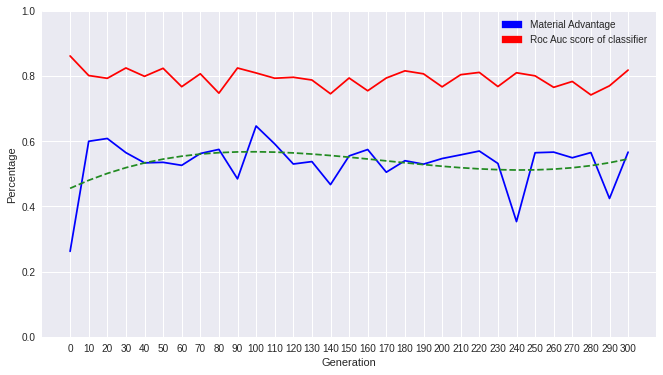
\includegraphics[width=0.7\textwidth]{graphics/number_pawns_trend}
    \caption{Percentage of selected states containing the HLC Material Advantage}
    \label{fig:numberadvantage}
\end{figure}

The Figure \ref{fig:numberadvantage}. shows that throughout training the Material Advantage HLC is only ever a slight factor in the selection of states and we can say that the neural network doesn't consider number advantage in its selection process.

\subsection{Agressiveness}

\begin{figure}[h]
    \centering
    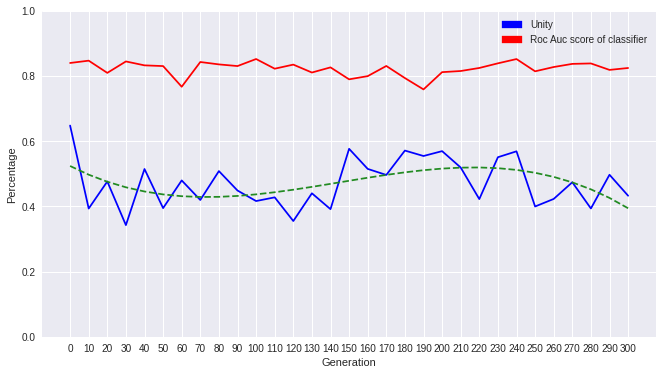
\includegraphics[width=0.7\textwidth]{graphics/most_advanced_trend.png}
    \caption{Percentage of selected states containing the HLC aggressiveness}
    \label{fig:aggressiveness}
\end{figure}

From Figure \ref{fig:aggressiveness}, we can see that the aggressiveness HLC is a growing factor over as the neural network is trained. As a piece can always move forward, if your opponent does not capture that piece, this concept relates to how many moves it will take for you to win. Generally, when your opponent is not playing well this concept does well, and quickly becomes a bad heuristic in classical search algorithms.

\subsection{Unity}

\begin{figure}[h]
    \centering
    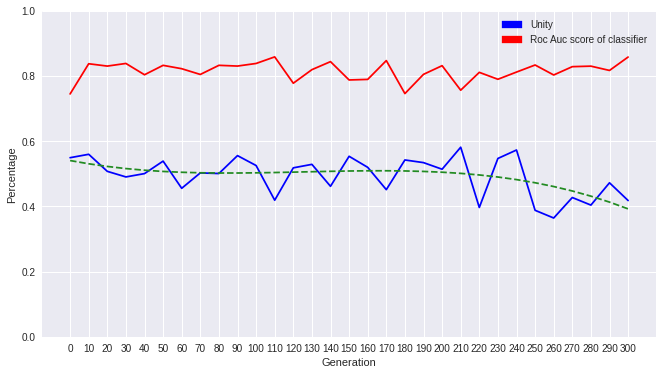
\includegraphics[width=0.7\textwidth]{graphics/unity_trend.png}
    \caption{Percentage of selected states containing the HLC unity}
    \label{fig:unity}
\end{figure}

Examining Figure \ref{fig:unity}, we see that the Unity HLC is steady, but then it drops as the network is trained. As this is considered a decent strategy in Breakthrough this is unexpected. However, this concept become increasingly unreliable as you lose pieces because it is the average of your remaining pieces distance to their center. 

\subsection{Lorentz-Horey Score}

\begin{figure}[h]
    \begin{small}
        \begin{center}
            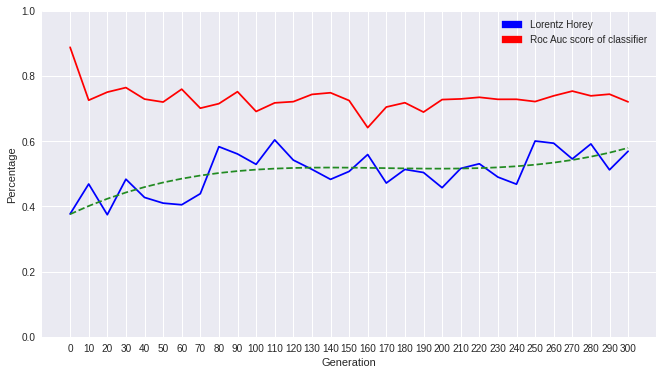
\includegraphics[width=0.95\textwidth]{graphics/lorentz_horey_trend.png}
        \end{center}
        \caption{Percentage of selected states containing the HLC Lorentz-Horey}
        \label{fig:lorentzheuristic}
    \end{small}
\end{figure}

Examining Figure \ref{fig:lorentzheuristic}, we can see a trend where as the neural network is trained its use of this HLC increases over time. As this heuristic is the one most often cited as a successful strategy in Breakthrough, it is interesting to see that our Breakthrough agent is gradually learning a similar concept.

\section{Summary}

In this section we discussed some concepts that we believed would be representative of concepts that a nerual network would learn over time playing Breakthrough. An important note is that there are an infinite amount of concepts, and there could exist some that the neural network uses extensively that we overlooked. We examined the neural network against these concepts. In the following chapter we will discuss the next steps for this research.%%RUM: "Results"
\chapter{Discussion}

This section discusses the results and the future work that could span from this research. Additionally, we conclude the work.

\section{Summary}

As seen in Chapter \ref{cha:results}, our trained agent does indeed quickly rise to using the higher-level concepts. The results are promising, as we see a popular concepts like Lorentz-Horey rise in emphasis for the neural network, and a simple but effective concept like Material Advantage rise slowly but not exessively. We find the Unity concept to be disappointing as stated earlier in this paper maintaining closeness of your pawns tends to be preferential. And lastly, for a the concept Aggressiveness, the fact that it falls off early is what we expected. It would have been the preferred result if we saw a greater variability in the concepts, but this could be a result from not enough training iterations, or not a complex enough model. Importantly, these concepts are only a few possibilities of an infinite set of concepts, and the neural network could be learning a completely different concept then those that we tested. However, that was not the focus of this research, it was to examine if a neural network does move towards HLC's that we humans use in games.

\section{Future Work}

To iterate on this research, training a neural network with greater computing power will allow the researchers to hopefully achieve a super-human neural network in Breakthrough. This would give a greater confidence in the learned concepts, possibly allowing for pedagological research on the topic regarding which concepts are optimal to train people in the game environment. This could also arise from a larger neural network architecture.

An avenue of research would be to use a trained AlphaZero model that plays chess to a super human ability, and be able to draw from a more diverse set of concepts. Furthermore, one could examine the play-style of the super-human model to extract concepts in order to construct new and improved heuristics for a non-neural network based agent.

Additionally applying this method to a greater set of environment would be an interesting field of research. We envision a self driving car agent being examined with respect to a higher level concept of aggressiveness, or a mortgage agent being examined with respect to a higher level concept of gender bias.

\section{Conclusion}

The work done in this paper is only a first step in examining working agents in active environments with respect to human level concepts. If improved could have a great impact in our trust on neural network that improve our daily lives. While the testbed for the research was a discrete game environment, there is a clear way forward to a dynamic system with discrete human level concepts. Our results show that for an agent that clearly doesn't achieve human level performance it's actions are often selected with respect to human level concepts, up to 60\% of the actions.
%%RUM: "Discussion"

%% ---------------------------------------------------------------
\printbibliography{} %%RUM: "References"

%% If appendices are needed, uncomment the following line
%% and include the appendices in separate files
\appendix{}%%RUM: "Appendicies (as appropriate)

%\backmatter{} % Sections after this don't get numbers
%% We prefer that all elements be numbered

%%%%%%%%%%%%% SHOW INDEX %%%%%%%%%%%%%%%%%%
%% Index, optional.  A good idea on longer documents

% You can put instructions at the beginning of the index:
%\renewcommand{\preindexhook}{%
%  The first page number is usually, but not always,
%  the primary reference to the indexed topic.\vskip\onelineskip}

%% You may have to run "makeindex <FILENAME>" to have it be generated
%% Depending upon which package you chose.
%%
\clearforchapter{}
\printindex{}%%RUM: Not mentioned

%\backcover{}%%RUM: "Back cover (only Phd)
\end{document}

%% ---------------------------------------------------------------

%%% Local Variables:
%%% mode: latex
%%% TeX-master: t
%%% TeX-engine: xetex
%%% End:
